% 2022 新高考Ⅱ卷 3：中国古建筑「举架」结构（简化示意图）
% 原图为木构屋架写实线描，此处按简化示意重绘，不追求写实细节，只保留题意所需的阶梯关系：
% 底部大梁之上叠三层逐层收短的横梁，层间以瓜柱（短柱）支撑，梁端置桁（檩）。
% 相邻桁的水平距离（步）恒取 1，瓜柱高（举）自下而上取 0.5、0.7、0.8、0.9，
% 故屋面折线呈上陡下缓。右半侧自上而下标桁位 A'、B'、C'、D'，其正下方梁上对应点标 A、B、C、D，
% 竖直段 AA'、BB'、CC'、DD' 即「举」，相邻两点的水平间距即「步」。
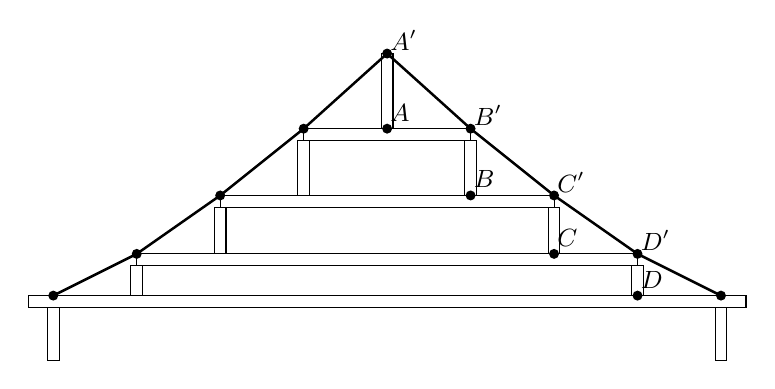
\begin{tikzpicture}[scale=1.06, font=\small]
  % ---- 梁：自下而上逐层收短（细长矩形示木料截面）----
  \draw (-4.3,-0.14) rectangle (4.3,0);
  \draw (-3,0.36)    rectangle (3,0.5);
  \draw (-2,1.06)    rectangle (2,1.2);
  \draw (-1,1.86)    rectangle (1,2.0);
  % ---- 檐柱（示意落地）----
  \draw (-4.07,-0.78) rectangle (-3.93,-0.14);
  \draw (3.93,-0.78)  rectangle (4.07,-0.14);
  % ---- 瓜柱：层间短柱，其高即「举」----
  \foreach \s in {-1,1}{
    \draw (3*\s-0.07,0)   rectangle (3*\s+0.07,0.36);
    \draw (2*\s-0.07,0.5) rectangle (2*\s+0.07,1.06);
    \draw (\s-0.07,1.2)   rectangle (\s+0.07,1.86);
  }
  \draw (-0.07,2.0) rectangle (0.07,2.9);          % 脊瓜柱
  % ---- 屋面折线：依次过各桁位 ----
  \draw[line width=0.9pt]
    (-4,0) -- (-3,0.5) -- (-2,1.2) -- (-1,2.0) -- (0,2.9)
           -- (1,2.0) -- (2,1.2) -- (3,0.5) -- (4,0);
  % ---- 桁位标记 ----
  \foreach \p in {(-4,0),(-3,0.5),(-2,1.2),(-1,2.0),(0,2.9),(1,2.0),(2,1.2),(3,0.5),(4,0)}
    { \fill \p circle (1.7pt); }
  \foreach \p in {(0,2.0),(1,1.2),(2,0.5),(3,0)} { \fill \p circle (1.7pt); }
  % ---- 标注（右半侧）----
  \node[above right, inner sep=1pt] at (0,2.9) {$A'$};
  \node[above right, inner sep=1pt] at (1,2.0) {$B'$};
  \node[above right, inner sep=1pt] at (2,1.2) {$C'$};
  \node[above right, inner sep=1pt] at (3,0.5) {$D'$};
  \node[above right, inner sep=1pt, yshift=1.5pt] at (0,2.0) {$A$};
  \node[above right, inner sep=1pt, yshift=1.5pt] at (1,1.2) {$B$};
  \node[above right, inner sep=1pt, yshift=1.5pt] at (2,0.5) {$C$};
  \node[above right, inner sep=1pt, yshift=1.5pt] at (3,0)   {$D$};
\end{tikzpicture}
